

\section{System Architecture}

\begin{figure}[ht!]
\centering
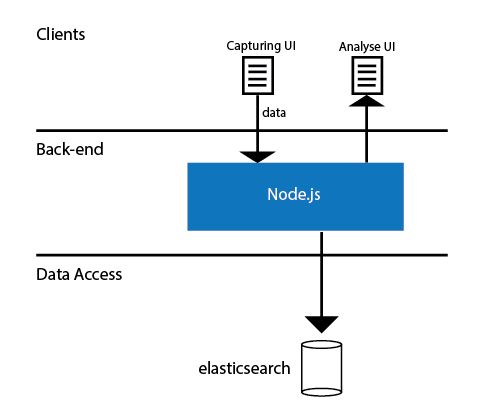
\includegraphics[width=100mm]{images/general/arhitecture.png}
\caption{Overall arhitecture of the system }
\label{overflow}
\end{figure}

The system architecture can be layered in to three layers; client, back-end, database. The control flow flows from the clients requesting something or inserting data, to the back-end and to the third layer, the database, and back up again in reverse order. 



\subsubsection{Interface}

The Soccer Analytic tool has one user interface - the web browser interface. Both the input and the analytic interface can be reached from this single web browser interface.

\subsubsection{Back-end}

The back-end is the middle layer between the client and the storage. Its main task is to serve static files to the clients, handle data insertions or handling web request by mapping them to database operations. New data insertions will possible be inserted into several database indexes. The back-end will then ensure that all indexes are updated before returning success to the client.

\subsubsection{Storage}

The storage layers task is to persist data and handle search queries on the data. It consist of several indexes that each store a part of domain model. 

\subsection{Domain model}

The domain model is based around matches. All attacks is wrapped into a match root. Attacks can be seen as subdocuments of the match document. Inside the attacks all passes lies with other information. This gives a easy way of understanding how all the data is related together. Below is a complete example of how it all is structured. The number of attacks and passes is stripped down to one in the example.

\lstinputlisting{domainmodel.js}

\section{Implementation details}

\begin{figure}[ht!]
\centering
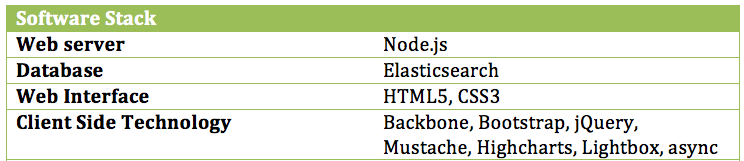
\includegraphics[width=100mm]{images/implementation/software_stack.png}
\caption{Software stack}
\label{overflow}
\end{figure}

\subsection{Storage}

The data storage is an elasticsearch database\cite{elasticsearch:mainsite}. Elasticsearch is document oriented, schemaless and works extremely well with JSON. As our server is built on JavaScript working with JSON is easy. JSON-objects can be inserted right into the storage and elasticsearch will map fields and value accordingly. 
Elasticsearch takes advantages of embedded documents meaning we can store related data together. As an attack is usually made up of several passes. With elasticsearch you can store the passes as an embedded document embedded in the attack document so they can be retrieved in one query. 

The main reason for using Elasticsearch is its search capability. In a single, simple to write query you can get counted how many passes all player for a team has played and received, number of times all players has been the breakthrough-player, type of attacks, most used zones for passing and finishing and so on. This makes it very easy and efficient to do queries for analyses on teams and players.  

\subsubsection{Indexes}



\subsection{Back-end}

The back end is the middle-ware between the clients and the data layer. It exposes a RESTful interface over HTTP for the client to communicate. A request coming in is transformed to a database query based on the resource it tries to access. On answer from the database the result is transformed before returning it to the client. 

Similar if the client sends new data for a match the middle-ware inserts the data into the appropriate indexes. The server will respond will HTTP status code 201 if all goes well or 400 on an error. The server uses HTTP code actively to tell the client the result of requests.

In principal, since the data input is generated in the web browser (with JavaScript), it could have been inserted right away into the database without going through an extra middleware. However, this limits us as we cant combine multiple queries by going through the back-end. Cleaning of data before serving to the client would neither be possible. Normally you also do validation of the data at the back-end before inserting into your database.

\subsubsection{API}

\begin{figure}[ht!]
\centering
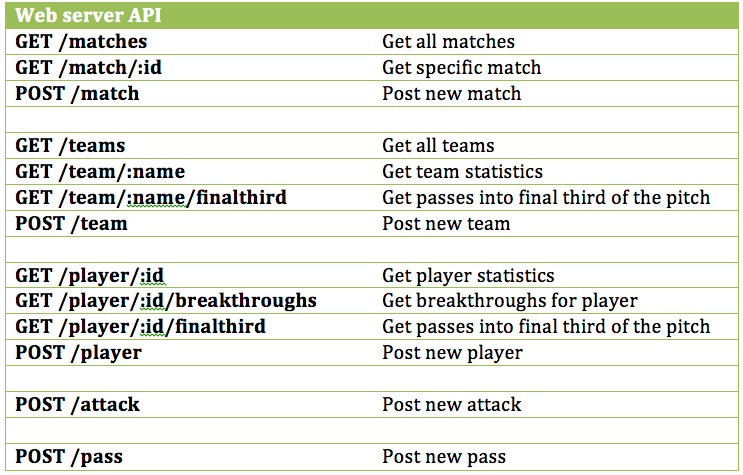
\includegraphics[width=100mm]{images/implementation/API.png}
\caption{Overview of the web servers API}
\label{overflow}
\end{figure}

\subsection{Front-end}

Front end is consist of a single page JavaScript application using Backbone.js as under-supporting framework. Backbone uses a MVC model to structure the code. With Backbone your views will update automatic when data changes. In the following sections the architecture of the client and how different concepts is used will be described. 

\begin{figure}[ht!]
\centering
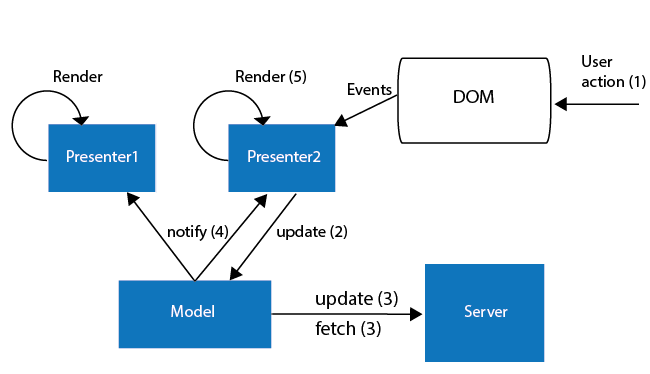
\includegraphics[width=150mm]{images/architecture/backbone_architecture.png}
\caption{Architecture of the client side}
\label{overflow}
\end{figure}

\subsubsection{Models}

Data is represented as models in backbone. The model has mainly to responsibilities. First is whenever a update on a models data occurs the model notifies the views that has subscribed for update events for that particular model. The second is that models is responsible for AJAX communication  with the back-end. An example is when a user creates registrates a new attack for a match. He fills out a form and press submit. Then a new Attack Model is created. Calling save on the instance of the model will send an AJAX post request to the server with the models data in the HTTP body.

Similar to a Attack Model we have Player Model that handles everything around players. When you click yourself into a players profile the model will fetch statistics from the back-end, notify the view that the data is ready, and the view will be rendered.

There is also a Match Model (fetching and registrating matches), Team Model (viewing statistics), and a Pass Model (saving passes). They work it the same way as the models described above.

\subsubsection{Views}

For a analytic toolkit to be useful a good UI is critical. Here several helper library is used to present the data. Highcharts.js is JavaScript library for illustrating graphs \cite{}. A query on team generates a lot of statistics and rather than listing them up they are presented using charts. This also gives us the advantage of displaying several numbers for each player and plot it in the same graph. In the image below we show the number of times a player has been involved in all attacks, number of passes into the final third of the pitch and the number of times a player has been the breakthrough-player.

\begin{figure}[ht!]
\centering
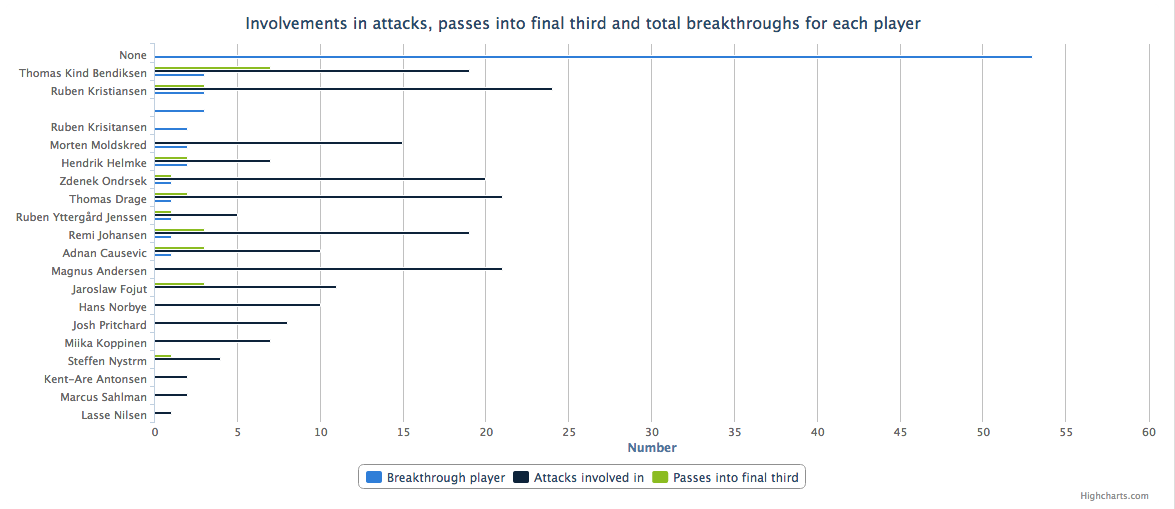
\includegraphics[width=100mm]{images/general/chart_passes.png}
\caption{Shows how the passing statistic is illustrated on the client by using Highcharts.js}
\label{overflow}
\end{figure}

Positional data is created using the a new feature of HTML5, canvases. From the model you get all zones with a number that symbols shots taken from that zone. This is then plotted into the respective zones. 

\begin{figure}[ht!]
\centering
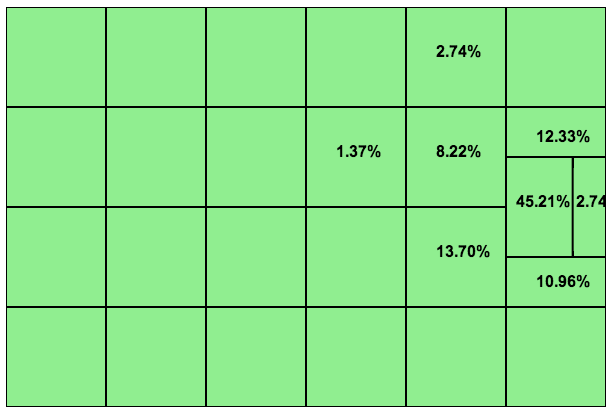
\includegraphics[width=85mm]{images/general/finishing_zones.png}
\caption{Illustrations of which zones the team has finished off their attacks from, with percent (team: Tromsø IL)}
\label{overflow}
\end{figure}

Backbone comes with a library Underscore.js that makes creating HTML pages with dynamic content easily. When you rending a new page on the site you can insert content retried from a model into the HTML and then render it.



\subsubsection{Security}
Secturity is not taken into convern. This means anyone getting into the page can post new match data. 